% Template last modified by Jake Hart; please contact course staff if you have any questions regarding using this template

\documentclass{cisXXX} % You must have the cisXXX .cls file in your project or working directory (i.e. the same directory as this document) 

\HWauthor{Zeyu Zhao}{zhaozeyu@seas.upenn.edu} % Put your name and Penn email on this line
\HWno{13} % Enter the number of the homework you are working on
\HWcourse{ESE 303} % Enter the course department and number here
%\HWpartner{Paul Brown} % If your class allows group work, put your partners here
%\HWpartner{Amelia Earhart} % Otherwise, delete or comment these lines 
\usepackage{amsmath}
\usepackage{amsfonts}
% code
\usepackage{color}
\usepackage[framed,numbered,autolinebreaks,useliterate]{mcode}
\usepackage{graphicx}
\definecolor{dkgreen}{rgb}{0,0.6,0}
\definecolor{gray}{rgb}{0.5,0.5,0.5}
\definecolor{mauve}{rgb}{0.58,0,0.82}
\begin{document}
\maketitle
\HWproblem
The $Y_t(s)$ is a Gaussian process because it is stated in (1) that $Y_t(s)$ is normally distributed with mean $\mu s$ and variance $\sigma^2s$.

Since we assume that $Y_t(s)$ over disjoint time intervals are independent, we know that for any $Y _ { n _ { 1 } }$ and $Y _ { n _ { 2 } } , n _ { 1 } \neq n _ { 2 }$, the time intervals $\left( n _ { 1 } , n _ { 1 } + h \right)$ and $\left( n _ { 2 } , n _ { 2 } + h \right)$ are disjoint, we know that they are independent. 

Using the above fact and from (2) that $Y _ { n } = Y _ { ( n - 1 ) h } ( h )$, we plug (2) into (1) and get that $Y_n$ is with mean $\mu h$ and variance $\sigma^2h$.

Therefore all $Y_n$ are i.i.d, each with mean $\mu h$ and variance $\sigma^2h$.
\HWproblem
We compute drift and volatility in MATLAB as follows:
\lstinputlisting{drift_volatility.m}

And we get output Figure \ref{fig:B1}.
\begin{figure}
	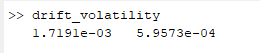
\includegraphics[width=\linewidth]{B.png} 
	\caption{Drift and Volatility} 
	\label{fig:B1}
\end{figure}

We obtain $\hat { \mu } = 1.7191 \times 10 ^ { - 3 }$ and $\hat { \sigma } ^ { 2 } = 5.9573 \times 10 ^ { - 4 }$.

\HWproblem
We use the following MATLAB code to compare the histogram with the computed PDFs and the CDFs:
\lstinputlisting{Y_n_sim_model.m}

The plots are shown in Figure \ref{fig:C1} and Figure \ref{fig:C2}.

\begin{figure}
  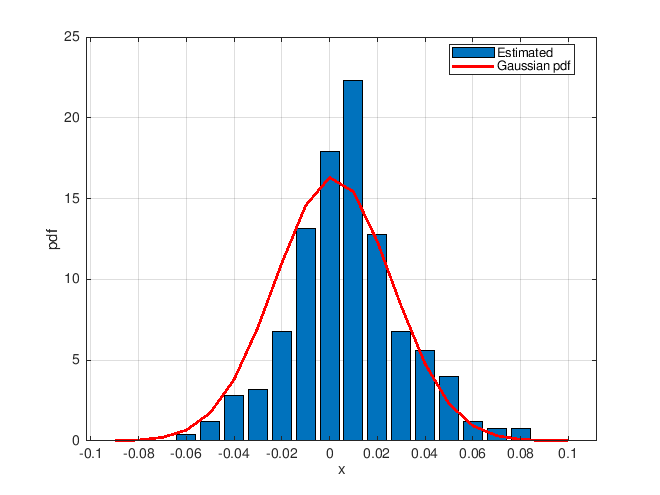
\includegraphics[width=\linewidth]{C1.png}
\caption{PDF of estimated $Y_n$ to normal model} 
  \label{fig:C1}
\end{figure}

\begin{figure}
  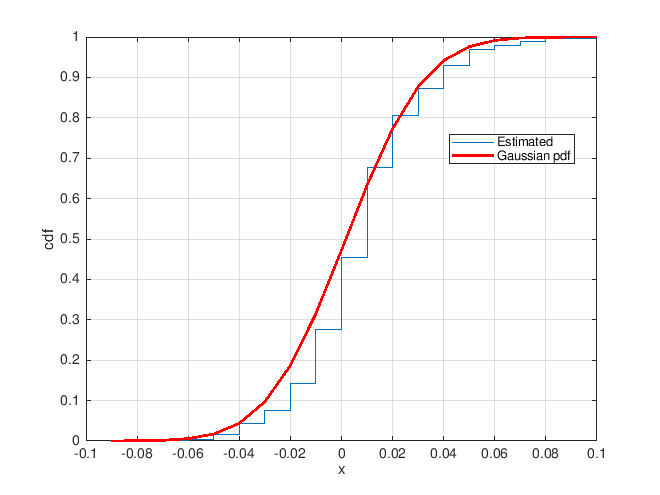
\includegraphics[width=\linewidth]{C2.png}
\caption{CDF of estimated $Y_n$ to normal model} 
  \label{fig:C2}
\end{figure}

Therefore, the geometric brownian motion model is an acceptable approximation. 
\HWproblem
Apply slide 27 of \textit{arbitrage\_stock\_and\_option\_pricing} on expected return and you can get the expected return for the stock:

$$
\begin{aligned} E _ { r } \left( t \right) & = e ^ { - \alpha t } \frac { \mathbb { E } [ X ( t ) | X ( 0 ) ] } { X ( 0 ) } \\ & = e ^ { \left( \hat { \mu } + \hat { \sigma } ^ { 2 } / 2 - \alpha \right) t } \end{aligned}
$$

Plugging in $\alpha = 0.1\%$ and the computed $\hat { \mu }, \hat { \sigma^2 }$, we get that 
$$ E _ { r } = e^{(1.7191*10^{-3} + 5.9573*10^{-4} / 2 -0.001) * 365} = 1.44946166$$.
So the rate of return is $145\%$.

The logarithm of $\frac { X ( t ) } { X ( 0 ) }$ follows a normal distribution with mean $\mu t$ and variance $\sigma^2 t$. Therefore,

$$
\begin{aligned} \mathbb { P } \left[ \frac { e ^ { - \alpha t } X ( t ) } { X ( 0 ) } \geq 1.05 \right] & = \mathbb { P } \left[ \log \left( \frac { e ^ { - \alpha t } X ( t ) } { X ( 0 ) } \right) \geq \log ( 1.05 ) \right] \\ & = \mathbb { P } \left[ \log \left( \frac { X ( t ) } { X ( 0 ) } \right) \geq \log ( 1.05 ) + \alpha t \right] \\ & = 1 - \Phi \left( \frac { \log ( 1.05 ) + \alpha t - \mu t } { \sqrt { \sigma ^ { 2 } t } } \right) \end{aligned},
$$
where $\Phi$ represents the cdf of the standard normal. Evaluating the value, we get that the probability is $0.63$.

\HWproblem

E Risk neutral measure. From slide 26 of \textit{arbitrage\_stock and\_option\_pricing}, the risk neutral measure refers to a rescaled geometric Brownian motion whose drift parameter is $\alpha - \sigma ^ { 2 } / 2$ and whose variance is $\sigma^2$. Plugging in the estimated values $\alpha = 0.001, \hat { \sigma } ^ { 2 } = 5.9573 \times 10 ^ { - 4 }$, we get the risk neutral measure for the CSCO stock is a geometric Brownian motion with mean $7.02 \times 10 ^ { - 4 } \cdot t$ and variance $5.96 \times 10 ^ { - 4 } \cdot t$.
\HWproblem
From the definition of risk neural mea- sure, it is ready that the expected discounted rate of return in the alternative reality is one (its logarithm is 0). Thus, the non-discounted rate of return is $\alpha$, i.e., the rate of return of the risk-free investment.
\HWproblem
The discounted expected return with respect to the risk neutral measure is:
$$
\mathbb { E } _ { q } \left[ e ^ { - \alpha t } [ X ( t ) - K ] _ { + } \right]
$$
From (7) and the fact that $c$ is deterministic, we know that the net gain with respect to the risk neutral measure is $0$. We may write as:
$$
\mathbb { E } _ { q } \left[ e ^ { - \alpha t } [ X ( t ) - K ] _ { + } - c \right] = 0
$$
which gives us $c(t)$:
$$
c ( t ) = e ^ { - \alpha t } \mathbb { E } _ { q } \left[ \left[ X ( 0 ) e ^ { Y ( t ) } - K \right] _ { + } \right]
$$
where $x ( t ) = x ( 0 ) e ^ { Y ( t ) }$ is a geometric brownian motion. This implies that $Y ( t )$ is normally distributed with parameters $\left( \mu t , \sigma ^ { 2 } t \right)$, and that:

$$
c ( t ) = e ^ { - \alpha t } \int _ { \log [ K / X ( 0 ) ] } ^ { \infty } \left( X ( 0 ) e ^ { y } - K \right) \exp \left[ - \frac { ( y - \mu t ) ^ { 2 } } { 2 \sigma ^ { 2 } t } \right] d y
$$
We simplify this equation with the steps listed in the course slides, and obtain the closed form of $c$:
$$
c = X ( 0 ) Q ( b ) - e ^ { - \alpha t } K Q ( a )
$$
where:
$$
\begin{aligned} a & = \frac { \log ( K ) - \log [ X ( 0 ) ] - \left( \alpha - \sigma ^ { 2 } / 2 \right) t } { \sqrt { \sigma ^ { 2 } t } } \\ b & = a - \sqrt { \sigma ^ { 2 } t } \end{aligned}
$$
\HWproblem
We first write a MATLAB function to determined the option price $c$ given a set of values of $k$.
\lstinputlisting{get_prices.m}
The plotting code in MATLAB:
\lstinputlisting{option_price.m}
The plots are shown in Figure \ref{fig:H1} and Figure \ref{fig:H2}.
From the plots:
Buying with $K = 1.2 * E [ X ( t ) ]$ corresponds to the situation where we would lose money by exercising our buying option. In this case, we would be better off purchasing the stock at the market price. However, buying at this price would still make sense if you expect volatility to favor us.
Buying with $K = 0.8 * E [ X ( t ) ]$ we expect to be able to resell the stock at increased price and make profit.

\begin{figure}
  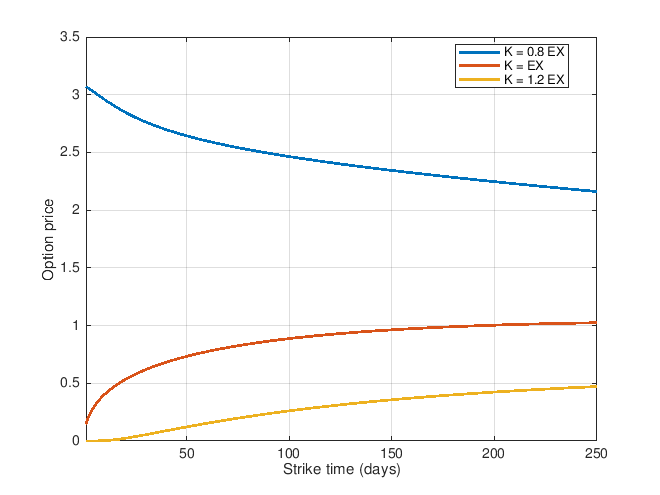
\includegraphics[width=\linewidth]{H1.png}
\caption{ option price } 
  \label{fig:H1}
\end{figure}

\begin{figure}
  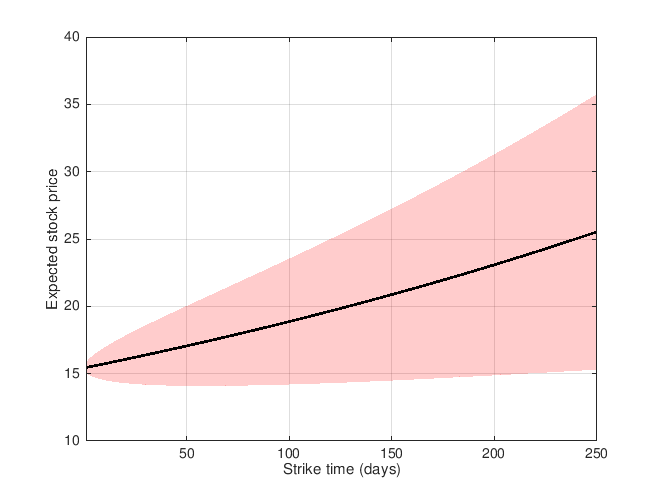
\includegraphics[width=\linewidth]{H2.png}
\caption{expected stock price with one standard deviation band} 
  \label{fig:H2}
\end{figure}
\end{document}